\documentclass{famnit-thesis}
% \documentclass[english]{famnit-thesis}       % For english version.
% \documentclass[cover]{famnit-thesis}         % Print the cover page.
% \documentclass[review]{famnit-thesis}        % The review version.
% \documentclass[english,cover]{famnit-thesis} % English version with the cover page.
% etc ...

% The bibliography is generated automatically through BibTex.
% Add the bibliography.bib file with all the bibtex entries.

% Import latex packages.
\usepackage{ccicons} % Remove if CC symbols are not needed.

% The basic thesis information.
\title
    {Naslov zaključne naloge}
    {The title of the final project paper}
    {Naslov v glavi dokumenta.}

\author{Ime}{Priimek}{I. Priimek}
\studyprogram{Računalništvo in informatika}
\mentor{prof. dr. Ime Mentorja}{Ime Mentorja, PhD}
\date{september}{2022}

% Additional thesis information. Remove if not used.
\comentor{doc. dr. Ime Somentorja}{Ime Somentorja, PhD}
\workingcomentor{dr. Ime Delovnega Somentorja}{Ime Delovnega Somentorja, PhD}

% List of keywords in Slovene and English language.
\keywords
    {beseda 1, beseda 2, beseda 3}
    {keyword 1, keyword2, keyword 3}

% Abstract in Slovene and English language.
\abstract
{
    Izvleček predstavlja kratek, a jedrnat prikaz vsebine
    naloge. V največ 250 besedah študent nakaže problem,
    metode, rezultate, ključne ugotovitve in njihov pomen.
}
{
    The abstract describes the content of the project work in a
    concise way. In no more than 250 words, the student outlines
    the problem, the methods, the results, and the conclusions.
}

% The acknowledgments.
\acknowledgments
{
    Zahvaljujem se \ldots
}

% An optional license page. Remove if not used.
\licensepage
{
    ~\vfill\noindent
    To delo je ponujeno pod licenco \emph{Creative Commons Priznanje avtorstva --- Deljenje} pod
    enakimi pogoji 2.5 Slovenija (ali novejšo različico). To pomeni, da se tako besedilo, slike,
    grafi in druge sestavine dela kot tudi rezultati diplomskega dela lahko prosto distribuirajo,
    reproducirajo, uporabljajo, priobčujejo javnosti in predelujejo, pod pogojem, da se jasno
    in vidno navede avtorja in naslov tega dela in da se v primeru spremembe, preoblikovanja
    ali uporabe tega dela v svojem delu, lahko distribuira predelava le pod licenco, ki je enaka
    tej. Podrobnosti licence so dostopne na spletni strani \url{http://creativecommons.si/} ali na
    Inštitutu za intelektualno lastnino, Streliška 1, 1000 Ljubljana.

    \begin{center}
        \Huge\ccbysa
    \end{center}
    
    \medskip\noindent
    Izvorna koda diplomskega dela, njeni rezultati in v ta namen razvita programska oprema je
    ponujena pod licenco GNU General Public License, različica 3 (alinovejša). To pomeni,
    da se lahko prosto distribuira in/ali predeluje pod njenimi pogoji. Podrobnosti licence so
    dostopne na spletni strani \url{http://www.gnu.org/licenses/}.
}

% The list of abbreviations. Remove if not used.
\abbreviation{SSH}{Secure Shell Protocol}
\abbreviation{SMTP}{Simple Mail Transfer Protocol}

\begin{document}
    % Thesis chapters.
    \chapter{UVOD}

Zaključna naloga je avtorsko delo, s katerim študent dokazuje poglobljeno znanje na širših
strokovnih in znanstvenih področjih, usposobljenost za iskanje novih virov znanja na
določenem strokovnem in znanstvenem področju, za uporabo znanstveno-raziskovalnih
metod v širšem spektru problemov in v novih ali spremenjenih okoliščinah, sposobnost za
prevzemanje odgovornosti za vodenje zahtevnejših delovnih sistemov ter za razvijanje
kritične refleksije.
    \chapter{Metodologija}

\noindent
Graf funkcije (\ref{eqn:saddle}) je prikazan na sliki \ref{fig:plot}.

\begin{equation}
    f(x, y) = x^2 - y^2
    \label{eqn:saddle}
\end{equation}

\begin{figure}[ht]
    \centering
    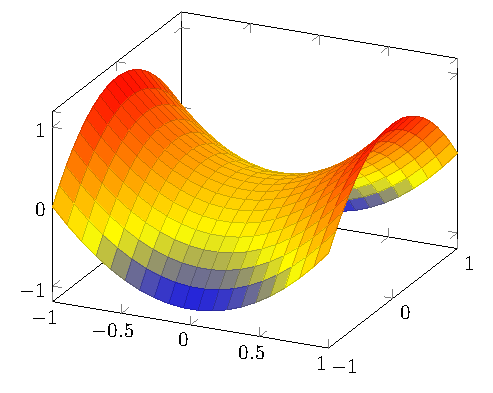
\includegraphics[width=0.6\linewidth]{images/plot.pdf}
    \caption{Graf funkcije $f(x, y) = x^2 - y^2$.}
    \label{fig:plot}
\end{figure}

\begin{table}[ht]
    \centering
    \caption{Nekaj vrednosti funkcije (\ref{eqn:saddle}).}
    \begin{tabular}{|rr|c|}
        \hline
        $x$  & $y$  & $f(x, y)$ \\
        \hline
        $-1$ & $-1$ & $0$ \\
        $-1$ & $0$  & $1$ \\
        $1$ & $0$   & $1$ \\
        \hline
    \end{tabular}
\end{table}

    % Optional appendices. Remove if not used.
    \appendix{A}{Naziv priloge}

Besedilo priloge.

\end{document}